\chapter{Seguimiento}
\label{chapter:seguimiento}
% Para cada tareas enumeradas en la fase de diseño y detalladas en la planificación, debes
% recoger los trabajos realizados, los problemas encontrados y las soluciones aplicadas, así
% como las posibles desviaciones que se han producido respecto a la planificación. Se puede
% crear una ficha por tarea que recoja toda la información.

\begin{table}[h!]
    \centering
\begin{tabularx}{\textwidth}{|>{\centering\arraybackslash}X|>{\centering\arraybackslash}X|}
\hline
\multicolumn{2}{|>{\columncolor[gray]{.8}}c|}{Tarea} \\ \hline
\multicolumn{2}{|c|}{Creación de las máquinas} \\ \hline
\rowcolor[gray]{.8} Tiempo planificado & Tiempo dedicado\\ \hline
30 minutos & 21 minutos\\ \hline
\rowcolor[gray]{.8} Problema & Solución\\ \hline
En Madrid no se pueden crear las máquinas N1 Micro.&Creamos las máquinas en Bélgica. A partir de ahora crearemos todas las máquinas en la misma zona para evitar problemas de conexión.\\ \hline
Las claves SSH hay que añadirlas en todas las máquinas&Leyendo la documentación veo que se puede añadir una clave SSH en el proyecto y se añadirá automáticamente a todas las máquinas. \\ \hline
\multicolumn{2}{|>{\columncolor[gray]{.8}}c|}{Actividad} \\ \hline
\multicolumn{2}{|p{0.95\linewidth}|}{Se crea una cuenta de Google Cloud Platform. Usaremos el proyecto por defecto para realizar las pruebas. En Compute Engine, en la pestaña de metadatos, añadimos la clave SSH de nuestro ordenador. Creamos las tres máquinas N1 Micro.
\begin{subfigure}{\textwidth}
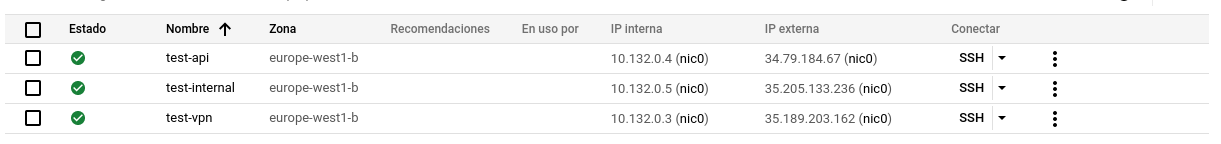
\includegraphics[width=0.95\textwidth]{figura6.png}
\caption{Máquinas virtuales creadas con sus IP asignadas automáticamente.}
\end{subfigure}
} 
\\ \hline
    \end{tabularx}
    \label{tab:tarea1}
\end{table}

\begin{table}[h!]
    \centering
\begin{tabularx}{\textwidth}{|>{\centering\arraybackslash}X|>{\centering\arraybackslash}X|}
\hline
\multicolumn{2}{|>{\columncolor[gray]{.8}}c|}{Tarea} \\ \hline
\multicolumn{2}{|c|}{Creación de la red} \\ \hline
\rowcolor[gray]{.8} Tiempo planificado & Tiempo dedicado\\ \hline
1 hora 30 minutos & 1 hora 24 minutos\\ \hline
\rowcolor[gray]{.8} Problema & Solución\\ \hline
El puerto de conexión SSH es público.&Si queremos acceder a la máquina desde cualquier ubicación con seguridad mantendremos esta configuración. Rechazaremos todo intento de conexión con contraseña. A cada servidor le daremos un puerto SSH al azar.\\ \hline
No es posible conectar con la máquina tras cambiar de puerto.&Se tiene que modificar el firewall de Google para poder acceder.\\ \hline
\multicolumn{2}{|>{\columncolor[gray]{.8}}c|}{Actividad} \\ \hline
\multicolumn{2}{|p{0.95\linewidth}|}{Nos conectamos por SSH a las tres máquinas para asegurarnos de su funcionamiento. Asignamos los siguientes puertos:
\begin{itemize}
    \item API: 47932/TCP.
    \item VPN: 18391/TCP
    \item Internal: 22899/TCP
\end{itemize}
Ahora, dentro de la configuración de las opciones de firewall, en el apartado Networking, debemos añadir una regla para permitir el acceso por el puerto SSH de cada máquina. A esta regla le debemos indicar una etiqueta. La misma etiqueta debe ponerse en las máquinas en las que se desee que se aplique la regla.
\begin{subfigure}{\textwidth}
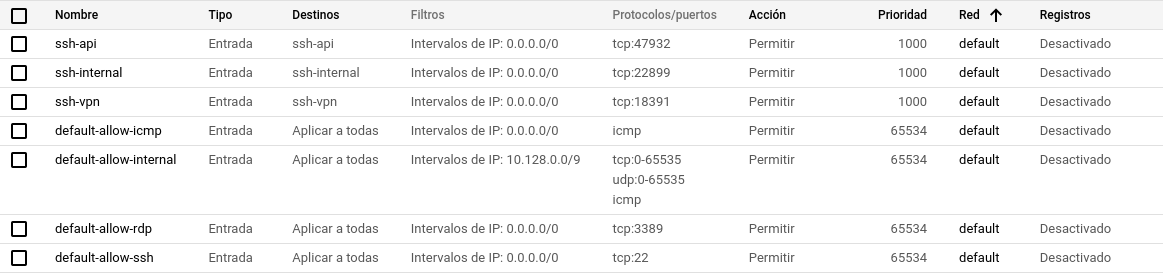
\includegraphics[width=0.95\textwidth]{figura7.png}
\caption{Reglas del firewall de Google. Las tres primeras son las que acabamos de añadir.}
\end{subfigure}

Tras estos cambios, accederemos al fichero de configuración del servicio SSH y lo modificaremos cambiando el puerto. Por defecto, Google ya realiza modificaciones en el fichero de forma que no se pueda acceder por contraseña ni se permita el acceso a root.

Cuando se crean las máquinas, Google les asigna una dirección IP privada estática para que puedan mantenerse en contacto entre ellas. Estas redes privadas solo las crea entre máquinas del mismo proyecto, por lo que separar las máquinas por proyectos facilita la organización en empresas grandes y seguriza el entorno haciendo que solo se vean entre si el mínimo número de máquinas.

Al tener las máquinas siempre encendidas, teóricamente, no nos debe preocupar el cambio de direcciones IP públicas. Igualmente, para evitar problemas, reservaremos una dirección IP para la conexión VPN. Esto se hace desde el panel de gestión de red VPC.
} 
\\ \hline
    \end{tabularx}
    \label{tab:tarea2}
\end{table}

\begin{table}[h!]
    \centering
\begin{tabularx}{\textwidth}{|>{\centering\arraybackslash}X|>{\centering\arraybackslash}X|}
\hline
\multicolumn{2}{|>{\columncolor[gray]{.8}}c|}{Tarea} \\ \hline
\multicolumn{2}{|c|}{VPN y subredes} \\ \hline
\rowcolor[gray]{.8} Tiempo planificado & Tiempo dedicado\\ \hline
3 horas 30 minutos & 2 horas 30 minutos\\ \hline
\rowcolor[gray]{.8} Problema & Solución\\ \hline
El script asigna al servidor una dirección aleatoria con máscara 24.&Para poder crear las subredes debemos modificar esto. El servidor debe aceptar /16. \\ \hline
Los clientes de la nueva máscara no tienen conexión.&Se debe modificar la regla iptables que hace referencia al enmascaramiento de la VPN para que aplique a la nueva máscara. \\ \hline
Al crear las subredes todos los departamentos pueden verse entre sí.&Debemos crear reglas en iptables para que solo sistemas pueda ver a otros departamentos.\cite{OpenVPNiptables} \\ \hline
\multicolumn{2}{|>{\columncolor[gray]{.8}}c|}{Actividad} \\ \hline
\multicolumn{2}{|p{0.95\linewidth}|}{Seguimos la documentación de PiVPN para instalar un servidor OpenVPN. El instalador ofrece una pequeña configuración. Para este proyecto introduciremos los siguientes datos:
\begin{itemize}
    \item Usuario en el que se guardarán las credenciales: [REDACTADO]
    \item Tipo de servidor: OpenVPN
    \item Configuración de puerto y protocolo por defecto (1194/UDP)
    \item Servidor DNS: Cloudflare (1.1.1.1)
    \item Verificamos que la dirección IP que nos indica es la correcta
    \item Uso de TSL-Crypt para mayor seguridad.
    \item Certificados RSA-256
    \item Actualizaciones automáticas habilitadas
\end{itemize}
En el siguiente paso abriremos el puerto 1194/UDP en el firewall de Google y creamos el primer usuario en la VPN para realizar la prueba. El script de instalación de PiVPN ha creado unos scripts dentro de \texttt{/usr/local/bin} para facilitarnos la gestión como si de un comando más se tratase. Usando el comando \texttt{pivpn add} generamos el nuevo usuario siguiendo los pasos que indica. Hemos podido comprobar que el cliente puede crear el túnel VPN y dispone de acceso a Internet a través de este.

El siguiente paso es crear un segundo usuario de VPN y probarlo en otro equipo. Si en el lado del servidor hemos aplicado las reglas iptables correspondientes al anexo \ref{anexo:iptables} seguiremos teniendo conexión a internet, pero cada equipo dispondrá de unos accesos concretos.

Cuando hemos realizado las comprobaciones, crearemos las credenciales de acceso para los otros servidores. Con el comando \texttt{pivpn add nopass} creamos credenciales sin contraseña de acceso. Esto es imprescindible si queremos que el servidor se conecte automáticamente sin interacción del usuario.} 
\\ \hline
    \end{tabularx}
    \label{tab:tarea3}
\end{table}

\begin{table}[h!]
    \centering
\begin{tabularx}{\textwidth}{|>{\centering\arraybackslash}X|>{\centering\arraybackslash}X|}
\hline
\multicolumn{2}{|>{\columncolor[gray]{.8}}c|}{Tarea} \\ \hline
\multicolumn{2}{|c|}{Controles de acceso} \\ \hline
\rowcolor[gray]{.8} Tiempo planificado & Tiempo dedicado\\ \hline
1 hora 30 minutos & 52 minutos \\ \hline
\rowcolor[gray]{.8} Problema & Solución\\ \hline
Si se cae la VPN no se puede acceder al servicio & La idea de esta restricción es justo que no pueda accederse sin la VPN, pero una norma del firewall de Cloudflare puede ser rápidamente modificada para permitir el acceso global de forma temporal. Si el acceso lo hubiésemos puesto usando registros DNS dentro de la VPN y la IP del túnel que comunica los servidores, habría sido mucho más costoso cualquier tipo de cambio.\\ \hline
\multicolumn{2}{|>{\columncolor[gray]{.8}}c|}{Actividad} \\ \hline
\multicolumn{2}{|p{0.95\linewidth}|}{Primero vamos a configurar el servidor Internal de dos maneras: Todo el personal tendrá acceso a los servicios y solo el departamento de sistemas podrá acceder a la administración.
Para el acceso \enquote{público} usaremos un túnel de Cloudflare, un servicio que nos permite realizar un proxy inverso sin necesidad de abrir puertos.
\begin{subfigure}{\textwidth}
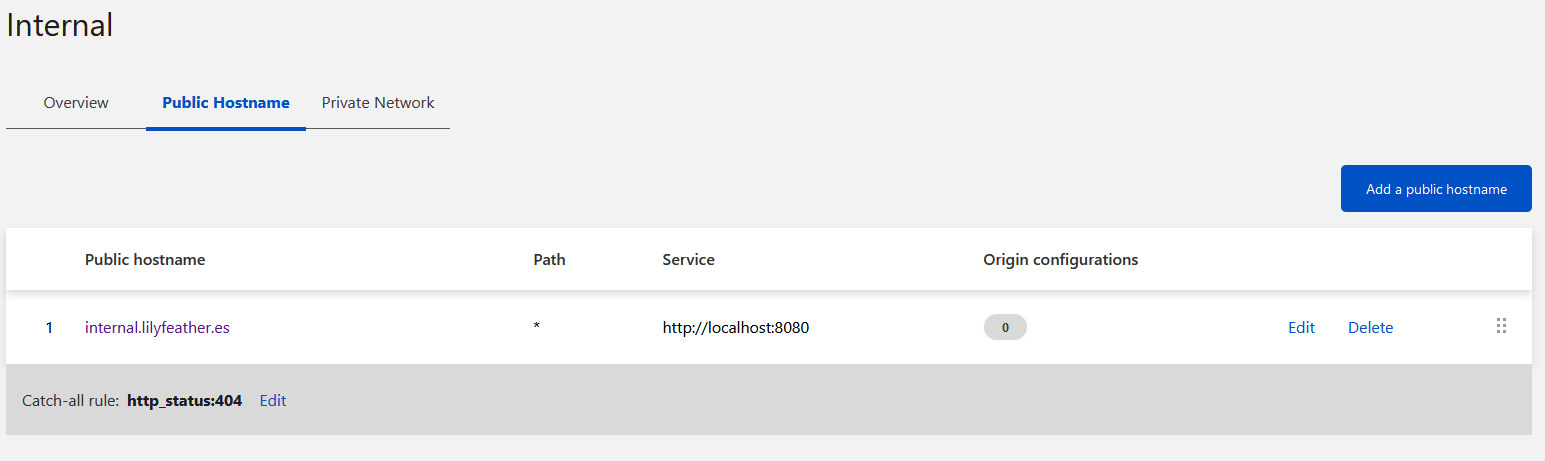
\includegraphics[width=0.95\textwidth]{figura8.png}
\caption{Tras la instalación del agente de Cloudflare en el servidor, indicamos el puerto de escucha y la entrada DNS se creará automáticamente.}
\end{subfigure}
Ahora que tenemos el servicio instalado y el DNS configurado, hay que indicar que solo se pueda acceder desde el servidor VPN.
\begin{subfigure}{\textwidth}
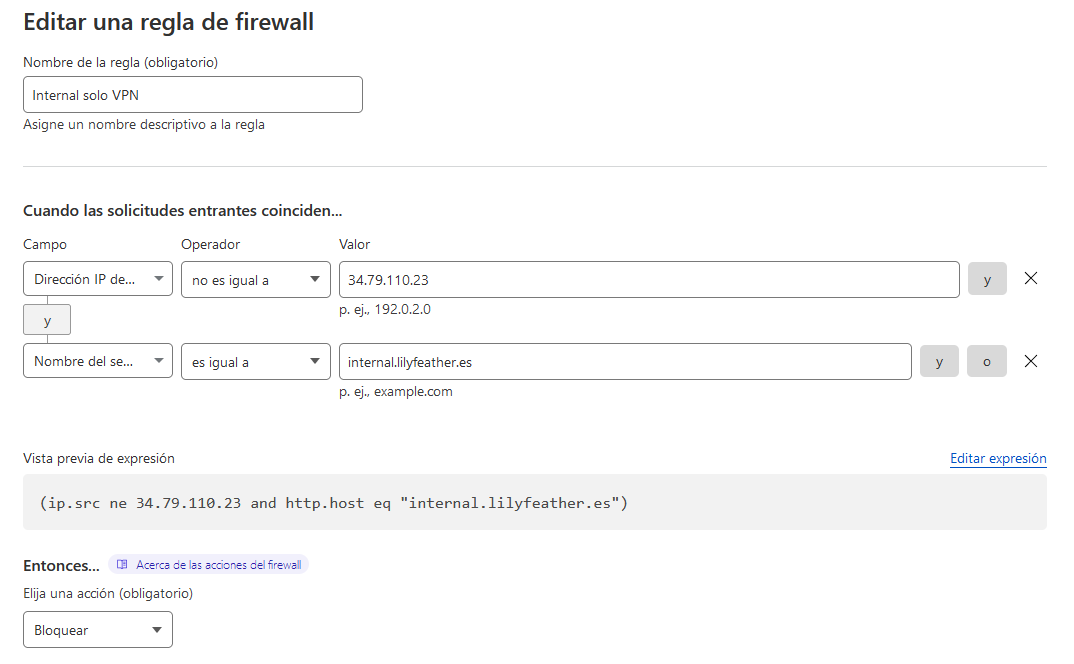
\includegraphics[width=0.95\textwidth]{figura9.png}
\end{subfigure}
Si en lugar de crear un túnel de Cloudflare decidimos abrir el puerto 443 al exterior, tendremos que añadir más medidas de seguridad. Si alguien descubre la IP pública del servidor y la añade a sus propios registros DNS, eludirá las reglas de Cloudflare. Para evitar esto habría que crear reglas iptables en el servidor Internal que rechacen toda conexión HTTPS que no proceda del proxy DNS de Cloudflare.

Para el servicio API creamos el mismo túnel pero sin restricciones.
}
\\ \hline
    \end{tabularx}
    \label{tab:tarea1}
\end{table}

\begin{table}[h!]
    \centering
\begin{tabularx}{\textwidth}{|>{\centering\arraybackslash}X|>{\centering\arraybackslash}X|}
\hline
\multicolumn{2}{|>{\columncolor[gray]{.8}}c|}{Tarea} \\ \hline
\multicolumn{2}{|c|}{Levantar servicios} \\ \hline
\rowcolor[gray]{.8} Tiempo planificado & Tiempo dedicado\\ \hline
30 minutos & 13 minutos\\ \hline
\rowcolor[gray]{.8} Problema & Solución\\ \hline
\multicolumn{2}{|>{\columncolor[gray]{.8}}c|}{Actividad} \\ \hline
\multicolumn{2}{|p{0.95\linewidth}|}{Dentro de la máquina Internal vamos a levantar un contenedor de Nextcloud. Docker nos ayudará a simplificar el proceso de implementación al igual que mejorará la seguridad tal y como se explica en el anexo \ref{anexo:docker}. Usaremos el archivo docker-compose disponible en el anexo \ref{anexo:docker-compose} para levantar los servicios necesarios. Esta configuración creará una red virtual con ambos contenedores. MariaDB solo podrá ser accesible desde el contenedor Nextcloud y el único acceso que se tendrá desde el exterior es un puerto redirigido.
} 
\\ \hline
    \end{tabularx}
    \label{tab:tarea1}
\end{table}

\begin{table}[h!]
    \centering
\begin{tabularx}{\textwidth}{|>{\centering\arraybackslash}X|>{\centering\arraybackslash}X|}
\hline
\multicolumn{2}{|>{\columncolor[gray]{.8}}c|}{Tarea} \\ \hline
\multicolumn{2}{|c|}{Segurizar servicios} \\ \hline
\rowcolor[gray]{.8} Tiempo planificado & Tiempo dedicado\\ \hline
1 hora & 45 minutos \\ \hline
\rowcolor[gray]{.8} Problema & Solución\\ \hline
1 hora & - \\ \hline
\multicolumn{2}{|>{\columncolor[gray]{.8}}c|}{Actividad} \\ \hline
\multicolumn{2}{|p{0.95\linewidth}|}{
La segurización de los servicios la hemos ido realizando de forma transversal en los anteriores puntos. Ahora nos enfocaremos en la seguridad pasiva de los servidores configurando las copias de seguridad. Primero, se programarán instantáneas de la máquina que alberga la VPN, de forma que los certificados y los logs estarán a salvo en caso de fallo, corrupción o ataque. La programación de snapshots se programa para todos los sábados entre las 2 y las 3 de la mañana y se almacenará redundantemente en todos los centros de datos de Europa.

Por otro lado, en la máquina Internal, se creará un cron que copie y comprima el contenido del directorio del contenedor Nextcloud, incluyendo el contenido de su almacenamiento y su base de datos, le dé un nombre descriptivo usando la fecha de creación, y suba el contenido al Bucket de Google usando su API.
} 
\\ \hline
    \end{tabularx}
    \label{tab:tarea1}
\end{table}
\begin{table}[h!]
Como hemos podido observar, el tiempo dedicado ha variado con respecto al planificado. Por ello, vamos a realizar una modificación del presupuesto relacionado con el personal técnico. Haciendo un sumatorio del las horas totales, el gasto final del personal técnico desciende a 212'91 € (6 horas).
\end{table}